% Options for packages loaded elsewhere
\PassOptionsToPackage{unicode}{hyperref}
\PassOptionsToPackage{hyphens}{url}
%
\documentclass[
]{book}
\usepackage{amsmath,amssymb}
\usepackage{iftex}
\ifPDFTeX
  \usepackage[T1]{fontenc}
  \usepackage[utf8]{inputenc}
  \usepackage{textcomp} % provide euro and other symbols
\else % if luatex or xetex
  \usepackage{unicode-math} % this also loads fontspec
  \defaultfontfeatures{Scale=MatchLowercase}
  \defaultfontfeatures[\rmfamily]{Ligatures=TeX,Scale=1}
\fi
\usepackage{lmodern}
\ifPDFTeX\else
  % xetex/luatex font selection
\fi
% Use upquote if available, for straight quotes in verbatim environments
\IfFileExists{upquote.sty}{\usepackage{upquote}}{}
\IfFileExists{microtype.sty}{% use microtype if available
  \usepackage[]{microtype}
  \UseMicrotypeSet[protrusion]{basicmath} % disable protrusion for tt fonts
}{}
\makeatletter
\@ifundefined{KOMAClassName}{% if non-KOMA class
  \IfFileExists{parskip.sty}{%
    \usepackage{parskip}
  }{% else
    \setlength{\parindent}{0pt}
    \setlength{\parskip}{6pt plus 2pt minus 1pt}}
}{% if KOMA class
  \KOMAoptions{parskip=half}}
\makeatother
\usepackage{xcolor}
\usepackage{color}
\usepackage{fancyvrb}
\newcommand{\VerbBar}{|}
\newcommand{\VERB}{\Verb[commandchars=\\\{\}]}
\DefineVerbatimEnvironment{Highlighting}{Verbatim}{commandchars=\\\{\}}
% Add ',fontsize=\small' for more characters per line
\usepackage{framed}
\definecolor{shadecolor}{RGB}{248,248,248}
\newenvironment{Shaded}{\begin{snugshade}}{\end{snugshade}}
\newcommand{\AlertTok}[1]{\textcolor[rgb]{0.94,0.16,0.16}{#1}}
\newcommand{\AnnotationTok}[1]{\textcolor[rgb]{0.56,0.35,0.01}{\textbf{\textit{#1}}}}
\newcommand{\AttributeTok}[1]{\textcolor[rgb]{0.13,0.29,0.53}{#1}}
\newcommand{\BaseNTok}[1]{\textcolor[rgb]{0.00,0.00,0.81}{#1}}
\newcommand{\BuiltInTok}[1]{#1}
\newcommand{\CharTok}[1]{\textcolor[rgb]{0.31,0.60,0.02}{#1}}
\newcommand{\CommentTok}[1]{\textcolor[rgb]{0.56,0.35,0.01}{\textit{#1}}}
\newcommand{\CommentVarTok}[1]{\textcolor[rgb]{0.56,0.35,0.01}{\textbf{\textit{#1}}}}
\newcommand{\ConstantTok}[1]{\textcolor[rgb]{0.56,0.35,0.01}{#1}}
\newcommand{\ControlFlowTok}[1]{\textcolor[rgb]{0.13,0.29,0.53}{\textbf{#1}}}
\newcommand{\DataTypeTok}[1]{\textcolor[rgb]{0.13,0.29,0.53}{#1}}
\newcommand{\DecValTok}[1]{\textcolor[rgb]{0.00,0.00,0.81}{#1}}
\newcommand{\DocumentationTok}[1]{\textcolor[rgb]{0.56,0.35,0.01}{\textbf{\textit{#1}}}}
\newcommand{\ErrorTok}[1]{\textcolor[rgb]{0.64,0.00,0.00}{\textbf{#1}}}
\newcommand{\ExtensionTok}[1]{#1}
\newcommand{\FloatTok}[1]{\textcolor[rgb]{0.00,0.00,0.81}{#1}}
\newcommand{\FunctionTok}[1]{\textcolor[rgb]{0.13,0.29,0.53}{\textbf{#1}}}
\newcommand{\ImportTok}[1]{#1}
\newcommand{\InformationTok}[1]{\textcolor[rgb]{0.56,0.35,0.01}{\textbf{\textit{#1}}}}
\newcommand{\KeywordTok}[1]{\textcolor[rgb]{0.13,0.29,0.53}{\textbf{#1}}}
\newcommand{\NormalTok}[1]{#1}
\newcommand{\OperatorTok}[1]{\textcolor[rgb]{0.81,0.36,0.00}{\textbf{#1}}}
\newcommand{\OtherTok}[1]{\textcolor[rgb]{0.56,0.35,0.01}{#1}}
\newcommand{\PreprocessorTok}[1]{\textcolor[rgb]{0.56,0.35,0.01}{\textit{#1}}}
\newcommand{\RegionMarkerTok}[1]{#1}
\newcommand{\SpecialCharTok}[1]{\textcolor[rgb]{0.81,0.36,0.00}{\textbf{#1}}}
\newcommand{\SpecialStringTok}[1]{\textcolor[rgb]{0.31,0.60,0.02}{#1}}
\newcommand{\StringTok}[1]{\textcolor[rgb]{0.31,0.60,0.02}{#1}}
\newcommand{\VariableTok}[1]{\textcolor[rgb]{0.00,0.00,0.00}{#1}}
\newcommand{\VerbatimStringTok}[1]{\textcolor[rgb]{0.31,0.60,0.02}{#1}}
\newcommand{\WarningTok}[1]{\textcolor[rgb]{0.56,0.35,0.01}{\textbf{\textit{#1}}}}
\usepackage{longtable,booktabs,array}
\usepackage{calc} % for calculating minipage widths
% Correct order of tables after \paragraph or \subparagraph
\usepackage{etoolbox}
\makeatletter
\patchcmd\longtable{\par}{\if@noskipsec\mbox{}\fi\par}{}{}
\makeatother
% Allow footnotes in longtable head/foot
\IfFileExists{footnotehyper.sty}{\usepackage{footnotehyper}}{\usepackage{footnote}}
\makesavenoteenv{longtable}
\usepackage{graphicx}
\makeatletter
\def\maxwidth{\ifdim\Gin@nat@width>\linewidth\linewidth\else\Gin@nat@width\fi}
\def\maxheight{\ifdim\Gin@nat@height>\textheight\textheight\else\Gin@nat@height\fi}
\makeatother
% Scale images if necessary, so that they will not overflow the page
% margins by default, and it is still possible to overwrite the defaults
% using explicit options in \includegraphics[width, height, ...]{}
\setkeys{Gin}{width=\maxwidth,height=\maxheight,keepaspectratio}
% Set default figure placement to htbp
\makeatletter
\def\fps@figure{htbp}
\makeatother
\setlength{\emergencystretch}{3em} % prevent overfull lines
\providecommand{\tightlist}{%
  \setlength{\itemsep}{0pt}\setlength{\parskip}{0pt}}
\setcounter{secnumdepth}{5}
\usepackage{booktabs}
\ifLuaTeX
  \usepackage{selnolig}  % disable illegal ligatures
\fi
\usepackage[]{natbib}
\bibliographystyle{plainnat}
\IfFileExists{bookmark.sty}{\usepackage{bookmark}}{\usepackage{hyperref}}
\IfFileExists{xurl.sty}{\usepackage{xurl}}{} % add URL line breaks if available
\urlstyle{same}
\hypersetup{
  pdftitle={Data Analysis in R: A Basic Guide},
  pdfauthor={Antonio Solorio},
  hidelinks,
  pdfcreator={LaTeX via pandoc}}

\title{Data Analysis in R: A Basic Guide}
\author{Antonio Solorio}
\date{2024-06-26}

\begin{document}
\maketitle

{
\setcounter{tocdepth}{1}
\tableofcontents
}
\hypertarget{introduction}{%
\chapter*{Introduction}\label{introduction}}
\addcontentsline{toc}{chapter}{Introduction}

Welcome to ``Data Analysis in R: A Basic Guide.'' This book aims to provide you with a basic foundation in data analysis using R, a powerful and versatile programming language. Throughout this book, you will learn various techniques and tools essential for effective data analysis.

To illustrate these concepts, we will use the Home Mortgage Disclosure Act (HMDA) data as a practical example. This real-world dataset will help you understand how to apply data analysis methods in a meaningful context.

\hypertarget{what-is-hmda-data}{%
\chapter{What is HMDA Data?}\label{what-is-hmda-data}}

The Home Mortgage Disclosure Act (HMDA) was enacted by Congress in 1975 and is implemented by the Consumer Financial Protection Bureau (CFPB). The HMDA requires many financial institutions to maintain, report, and publicly disclose information about mortgages. This information is crucial for understanding and monitoring trends in housing finance, and for ensuring compliance with fair lending laws. \footnote{If you would like to learn more about HMDA data please see: \url{https://www.consumerfinance.gov/data-research/hmda/}}

HMDA data includes information on loan applications, loan originations, loan purchases, and denied applications. The data encompasses various aspects such as:

\begin{itemize}
\tightlist
\item
  \textbf{Loan Characteristics}: Information about the loan amount, type of loan, and purpose of the loan (e.g., home purchase, refinance).
\item
  \textbf{Applicant Information}: Demographic details of the loan applicants including race, ethnicity, gender, and income.
\item
  \textbf{Property Information}: Data about the location and type of property being financed.
\item
  \textbf{Action Taken}: The outcome of the loan application, whether it was approved, denied, or withdrawn.
\end{itemize}

\hypertarget{why-use-hmda-data}{%
\section{Why Use HMDA Data?}\label{why-use-hmda-data}}

While this book is focused on teaching data analysis in R, the HMDA dataset serves as an excellent example for several reasons:

\begin{enumerate}
\def\labelenumi{\arabic{enumi}.}
\tightlist
\item
  \textbf{Real-World Relevance}: HMDA data provides a real-world context that makes the learning process more engaging and practical.
\item
  \textbf{Comprehensive Dataset}: The dataset includes a wide range of variables, making it suitable for demonstrating various data analysis techniques.
\item
  \textbf{Publicly Available}: HMDA data is publicly accessible, allowing you to follow along with the examples and practice on your own.
\end{enumerate}

By the end of this book, you will not only have a solid understanding of data analysis in R but also be equipped with practical skills that can be applied to other datasets and domains.

Let's get started on this journey of exploring data analysis with R, using the HMDA data as our guide!

\hypertarget{data-importing}{%
\chapter{Data Importing}\label{data-importing}}

In this chapter, we will explore the process of importing data into R for analysis. Data import is a crucial step in the data analysis workflow, as it allows you to load external data into R for further processing and analysis. We will focus on importing data from CSV files, which are one of the most common data formats used in data analysis. We will also discuss common issues encountered during data import and how to handle them, and how to handle the importation of large datasets in chunks.

\hypertarget{different-types-of-data}{%
\section{Different Types of Data}\label{different-types-of-data}}

In the realm of data analysis, you will encounter various types of data formats. Here are some common ones:

\begin{itemize}
\tightlist
\item
  \textbf{Text Files}: Unstructured text data that can be read line by line or in blocks, and which may be delimited by specific characters.
\item
  \textbf{CSV (Comma-Separated Values)}: A CSV file is a type of text file that is delimited by commas. It is one of the most common data formats used for storing tabular data.
\item
  \textbf{Excel Files}: Commonly used spreadsheets saved in formats like \texttt{.xlsx} or \texttt{.xls}.
\item
  \textbf{JSON (JavaScript Object Notation)}: A lightweight data interchange format that is easy for humans to read and write and easy for machines to parse and generate.
\item
  \textbf{SQL Databases}: Structured data stored in relational databases, which can be queried using SQL (Structured Query Language).
\item
  \textbf{API Data}: Data fetched from web APIs, which often come in formats like JSON or XML.
\end{itemize}

\hypertarget{why-start-with-csv-files}{%
\subsection{Why Start with CSV Files?}\label{why-start-with-csv-files}}

We will start with CSV files for several reasons:

\begin{enumerate}
\def\labelenumi{\arabic{enumi}.}
\tightlist
\item
  \textbf{Simplicity}: CSV files are easy to understand and work with, making them ideal for beginners.
\item
  \textbf{Ubiquity}: CSV is one of the most common data formats, widely supported by various applications and programming languages.
\item
  \textbf{Ease of Use in R}: R provides straightforward functions for importing and handling CSV files, making it an excellent starting point for learning data import techniques.
\end{enumerate}

By mastering the import of CSV files, you'll build a strong foundation that will make it easier to work with other data formats as you progress in your data analysis journey.

\hypertarget{downloading-and-importing-hmda-data-in-csv-format}{%
\section{Downloading and Importing HMDA Data in CSV Format}\label{downloading-and-importing-hmda-data-in-csv-format}}

To practice importing CSV files in R, we will use the Home Mortgage Disclosure Act (HMDA) data in CSV format. This data can be found at the \href{https://ffiec.cfpb.gov/}{Consumer Financial Protection Bureau (CFPB) website}. In particular we will be working with the Snapshot National Loan Level Dataset, specifically for that in 2022 for Nevada.

\hypertarget{snapshot-national-loan-level-dataset}{%
\subsection{Snapshot National Loan Level Dataset}\label{snapshot-national-loan-level-dataset}}

The Snapshot files contain the national HMDA datasets as of May 1, 2023 for all HMDA reporters, as modified by the Bureau to protect applicant and borrower privacy. The snapshot files are available to download in both .csv and pipe delimited text file formats at the following link: \url{https://ffiec.cfpb.gov/data-publication/snapshot-national-loan-level-dataset/}. One of the issues with these files however is that they are quite large, so we will be working with a subset of the data for Nevada in 2022.

The subset of the data for Nevada in 2022 can be downloaded from the following link: \href{https://ffiec.cfpb.gov/v2/data-browser-api/view/csv?states=NV\&years=2022}{Nevada 2022 HMDA Data}.

\hypertarget{importing-csv-files-in-r}{%
\section{Importing CSV Files in R}\label{importing-csv-files-in-r}}

R provides several functions for importing CSV files. The most commonly used function is \textbf{\texttt{read.csv()}}, which is part of the base R package. Additionally, the \textbf{\texttt{readr}} package offers the \textbf{\texttt{read\_csv()}} function, which is optimized for faster performance and easier handling of large datasets.

\hypertarget{using-read.csv}{%
\subsection{\texorpdfstring{Using \texttt{read.csv()}}{Using read.csv()}}\label{using-read.csv}}

The \textbf{\texttt{read.csv()}} function is straightforward to use. It is actually a special case of the more general \textbf{\texttt{read.table()}} function, with default parameters set for reading CSV files Here's how you can import a CSV file using this function:

\begin{Shaded}
\begin{Highlighting}[]
\CommentTok{\# Importing a CSV file using read.csv()}
\NormalTok{data }\OtherTok{\textless{}{-}} \FunctionTok{read.csv}\NormalTok{(}\StringTok{"downloads/state\_NV.csv"}\NormalTok{)}

\CommentTok{\# Display the first few rows of the data}
\FunctionTok{head}\NormalTok{(data)}
\end{Highlighting}
\end{Shaded}

In this example, replace \textbf{\texttt{"downloads/state\_NV.csv"}} with the actual path to your CSV file. The \textbf{\texttt{head()}} function is used to display the first few rows of the imported data.

\hypertarget{details-on-read.csv}{%
\subsubsection*{\texorpdfstring{Details on \texttt{read.csv()}}{Details on read.csv()}}\label{details-on-read.csv}}
\addcontentsline{toc}{subsubsection}{Details on \texttt{read.csv()}}

The \textbf{\texttt{read.csv()}} function is a simplified wrapper around \textbf{\texttt{read.table()}}, with pre-set arguments tailored for reading comma-separated files. Specifically, it sets the following default arguments:

\begin{itemize}
\tightlist
\item
  \textbf{\texttt{sep\ =\ ","}} sets the field separator to a comma.
\item
  \textbf{\texttt{header\ =\ TRUE}} indicates that the first line of the file contains column names.
\item
  \textbf{\texttt{stringsAsFactors\ =\ default.stringsAsFactors()}} specifies whether character vectors should be converted to factors (default behavior depends on the R version).
\end{itemize}

Here's an equivalent way to use \texttt{read.table()} to achieve the same result as \texttt{read.csv()}:

\begin{Shaded}
\begin{Highlighting}[]
\CommentTok{\# Importing a CSV file using read.table()}
\NormalTok{data }\OtherTok{\textless{}{-}} \FunctionTok{read.table}\NormalTok{(}\StringTok{"downloads/state\_NV.csv"}\NormalTok{, }\AttributeTok{sep =} \StringTok{","}\NormalTok{, }\AttributeTok{header =} \ConstantTok{TRUE}\NormalTok{, }\AttributeTok{stringsAsFactors =} \ConstantTok{FALSE}\NormalTok{)}

\CommentTok{\# Display the first few rows of the data}
\FunctionTok{head}\NormalTok{(data)}
\end{Highlighting}
\end{Shaded}

As you can see, read.csv() simplifies the process by encapsulating these common settings, making it easier and quicker to read CSV files.

\hypertarget{using-read_csv-from-the-readr-package}{%
\subsection{\texorpdfstring{Using \texttt{read\_csv()} from the \texttt{readr} Package}{Using read\_csv() from the readr Package}}\label{using-read_csv-from-the-readr-package}}

The \textbf{\texttt{readr}} package provides a faster and more convenient way to import CSV files with the \textbf{\texttt{read\_csv()}} function. First, you need to install and load the \textbf{\texttt{readr}} package:

\begin{Shaded}
\begin{Highlighting}[]
\CommentTok{\# Install the readr package}
\FunctionTok{install.packages}\NormalTok{(}\StringTok{"readr"}\NormalTok{)}
\end{Highlighting}
\end{Shaded}

Once the package is installed, you can use the \textbf{\texttt{read\_csv()}} function to import the CSV file:

\begin{Shaded}
\begin{Highlighting}[]
\CommentTok{\# Load the readr package}
\FunctionTok{library}\NormalTok{(readr)}

\CommentTok{\# Importing a CSV file using read\_csv()}
\NormalTok{data }\OtherTok{\textless{}{-}} \FunctionTok{read\_csv}\NormalTok{(}\StringTok{"downloads/state\_NV.csv"}\NormalTok{)}

\CommentTok{\# Display the first few rows of the data}
\FunctionTok{head}\NormalTok{(data,}\DecValTok{50}\NormalTok{)}
\end{Highlighting}
\end{Shaded}

Similar to \textbf{\texttt{read.csv()}}, replace \textbf{\texttt{"downloads/state\_NV.csv"}} with the actual path to your CSV file. The \textbf{\texttt{read\_csv()}} function also automatically parses the data types of the columns, which can save you time and effort, {you need to be carefull as sometimes read\_csv() may guess the column type wrong!}

\hypertarget{details-on-read_csv}{%
\subsection*{\texorpdfstring{Details on \texttt{read\_csv()}}{Details on read\_csv()}}\label{details-on-read_csv}}
\addcontentsline{toc}{subsection}{Details on \texttt{read\_csv()}}

The \textbf{\texttt{read\_csv()}} function is a special case of the more general \textbf{\texttt{read\_delim()}} function from the \textbf{\texttt{readr}} package, with default parameters set for reading comma-separated files. Specifically, it sets the following default arguments:

\begin{itemize}
\tightlist
\item
  \textbf{\texttt{delim\ =\ ","}} sets the field separator to a comma.
\item
  \textbf{\texttt{col\_types\ =\ cols()}} automatically detects the data types of columns unless specified otherwise.
\item
  \textbf{\texttt{trim\_ws\ =\ TRUE}} indicates that whitespace should be trimmed from the beginning and end of each field.
\end{itemize}

These defaults make \textbf{\texttt{read\_csv()}} particularly convenient for reading CSV files without needing to manually specify these common options.

Here's an equivalent way to use \textbf{\texttt{read\_delim()}} to achieve the same result as \textbf{\texttt{read\_csv()}}:

\begin{Shaded}
\begin{Highlighting}[]
\CommentTok{\# Importing a CSV file using read\_delim()}
\NormalTok{data }\OtherTok{\textless{}{-}} \FunctionTok{read\_delim}\NormalTok{(}
  \StringTok{"downloads/state\_NV.csv"}\NormalTok{,}
  \AttributeTok{delim =} \StringTok{","}\NormalTok{,}
  \AttributeTok{col\_types =} \FunctionTok{cols}\NormalTok{(),}
  \AttributeTok{trim\_ws =} \ConstantTok{TRUE}
\NormalTok{)}

\CommentTok{\# Display the first few rows of the data}
\FunctionTok{head}\NormalTok{(data, }\DecValTok{50}\NormalTok{)}
\end{Highlighting}
\end{Shaded}

As you can see, \textbf{read\_csv()} simplifies the process by encapsulating these common settings, making it easier and quicker to read CSV files.

\hypertarget{handling-parsing-issues}{%
\subsubsection{Handling Parsing Issues}\label{handling-parsing-issues}}

If you been following along, when you ran \textbf{\texttt{data\ \textless{}-\ read\_csv("downloads/state\_NV.csv")}} you have probably encountered a {warning} similar to:

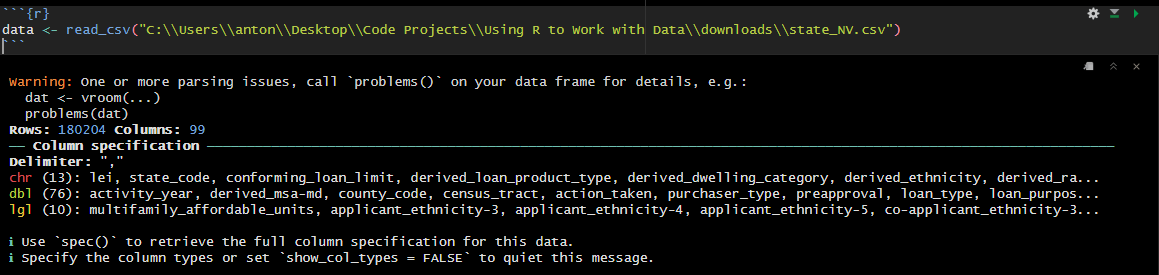
\includegraphics{images/clipboard-3586307356.png}

The warning is letting us know that \textbf{\texttt{read\_csv()}} ran into some parsing issues, and its recommending that we run \textbf{\texttt{problems()}} to see what the issues are. Let's run \textbf{\texttt{problems()}} to see what the issues are:

\begin{Shaded}
\begin{Highlighting}[]
\CommentTok{\# Display the problems encountered during parsing}
\FunctionTok{problems}\NormalTok{(data)}
\end{Highlighting}
\end{Shaded}

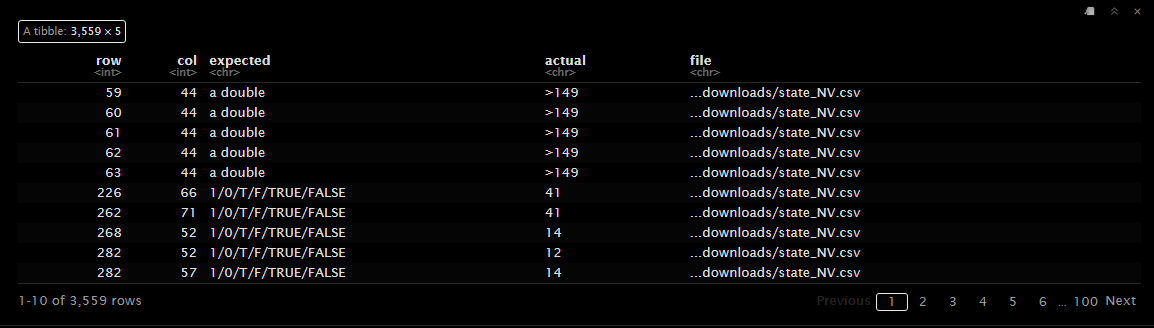
\includegraphics{images/clipboard-1927136276.png}

The \textbf{\texttt{problems()}} function displays the issues encountered during parsing. The \textbf{`row'} column indicates the row number where the issue occurred, and the \textbf{`col'} column indicates the column number. The \textbf{`expected'} column shows the expected data type, and the \textbf{`actual'} column shows the actual value.

There are two main ways to handle parsing issues in \texttt{read\_csv()}:

\begin{itemize}
\tightlist
\item
  \textbf{Manually Specify Column Types}: You can manually specify the column types using the \texttt{col\_types} argument in \textbf{\texttt{read\_csv()}}. This approach is useful when you know the data types of the columns in advance, but might be cumbersome for large datasets with many columns.
\item
  \textbf{Increase the \texttt{guess\_max} Argument}: You can increase the \texttt{guess\_max} argument in \texttt{read\_csv()} to allow the function to guess the column types for a larger number of rows. This approach isn't perfect, but this way you can avoid having to manually specify the column types.
\end{itemize}

Below is the code to manually specify the column types:

\begin{Shaded}
\begin{Highlighting}[]
\CommentTok{\# Manually specify the column types}
\NormalTok{data }\OtherTok{\textless{}{-}} \FunctionTok{read\_csv}\NormalTok{(}
  \StringTok{"C:}\SpecialCharTok{\textbackslash{}\textbackslash{}}\StringTok{Users}\SpecialCharTok{\textbackslash{}\textbackslash{}}\StringTok{anton}\SpecialCharTok{\textbackslash{}\textbackslash{}}\StringTok{Desktop}\SpecialCharTok{\textbackslash{}\textbackslash{}}\StringTok{Code Projects}\SpecialCharTok{\textbackslash{}\textbackslash{}}\StringTok{Using R to Work with Data}\SpecialCharTok{\textbackslash{}\textbackslash{}}\StringTok{downloads}\SpecialCharTok{\textbackslash{}\textbackslash{}}\StringTok{state\_NV.csv"}\NormalTok{,}
  \AttributeTok{col\_types =} \FunctionTok{cols}\NormalTok{(}
    \AttributeTok{loan\_amount =} \FunctionTok{col\_double}\NormalTok{(),}
    \AttributeTok{total\_units =} \FunctionTok{col\_character}\NormalTok{(),}
    \AttributeTok{.default =} \FunctionTok{col\_character}\NormalTok{(),}
\NormalTok{  ),}
  \AttributeTok{na =} \FunctionTok{c}\NormalTok{(}\StringTok{""}\NormalTok{, }\StringTok{"NA"}\NormalTok{) }\CommentTok{\# This is to specify what is considered a missing value}
\NormalTok{  )}
\end{Highlighting}
\end{Shaded}

\hypertarget{handling-file-paths}{%
\subsection{Handling File Paths}\label{handling-file-paths}}

When specifying the path to your CSV file, it's important to ensure that the path is correct. You can use absolute paths or relative paths. Here are some examples:

\begin{itemize}
\tightlist
\item
  \textbf{Absolute Path}: An absolute path specifies the complete path from the root directory. For example, on Windows: \texttt{"C:/Users/YourName/Documents/data.csv"}, or on macOS/Linux: \texttt{"/Users/YourName/Documents/data.csv"}.
\item
  \textbf{Relative Path}: A relative path specifies the path relative to your current working directory. For example, if your current working directory is \texttt{"C:/Users/YourName/Documents"}, you can use \texttt{"data.csv"}.
\end{itemize}

You can check your current working directory in R using the \texttt{getwd()} function:

\begin{Shaded}
\begin{Highlighting}[]
\CommentTok{\# Get the current working directory}
\FunctionTok{getwd}\NormalTok{()}
\end{Highlighting}
\end{Shaded}

You can also set the working directory using the \texttt{setwd()} function:

\begin{Shaded}
\begin{Highlighting}[]
\CommentTok{\# Set the working directory}
\FunctionTok{setwd}\NormalTok{(}\StringTok{"path/to/your/directory"}\NormalTok{)}
\end{Highlighting}
\end{Shaded}

\hypertarget{common-issues-and-solutions}{%
\subsection{Common Issues and Solutions}\label{common-issues-and-solutions}}

\begin{itemize}
\tightlist
\item
  \textbf{File Not Found Error}: Ensure the file path is correct and the file exists at the specified location.
\item
  \textbf{Incorrect Data Parsing}: If columns are not parsed correctly, you can specify the column types manually using the \texttt{col\_types} argument in \texttt{read\_csv()}.
\item
  \textbf{Missing Values}: R automatically handles missing values as \texttt{NA}. You can customize the handling of missing values using the \texttt{na} argument.
\end{itemize}

By understanding how to import CSV files in R, you can easily load your data and start your data analysis process. In the next sections, we will explore how to clean and manipulate the imported data to prepare it for analysis.

\newpage

\hypertarget{importing-data-in-chunks}{%
\section{Importing Data in Chunks}\label{importing-data-in-chunks}}

When working with large datasets, it's often necessary to import data in chunks, especially when the dataset is too large to fit into memory or cannot be opened by standard software like Excel. The readr package in R provides a solution with the \textbf{\texttt{read\_delim\_chunked()}} function, which allows for reading a delimited file in manageable chunks.

The \textbf{\texttt{read\_delim\_chunked()}} function operates similarly to \textbf{\texttt{read\_delim()}}, but it processes data in smaller portions, making it easier to handle large datasets. A practical approach is to use a callback function to filter data as each chunk is processed.

Here's an example demonstrating how to import a delimited file in chunks and apply a callback function to filter the data for state\_code ``NV'':

\begin{Shaded}
\begin{Highlighting}[]
\CommentTok{\# Load the readr package}
\FunctionTok{library}\NormalTok{(readr)}
\FunctionTok{library}\NormalTok{(dplyr)}

\CommentTok{\# Define the callback function to filter data for state\_code "NV"}
\NormalTok{filter\_data }\OtherTok{\textless{}{-}} \ControlFlowTok{function}\NormalTok{(data\_chunk, pos) \{}
  \CommentTok{\# Filters data chunk for only rows where state\_code == "NV"}
\NormalTok{  data\_chunk }\OtherTok{\textless{}{-}}\NormalTok{ data\_chunk}\SpecialCharTok{\%\textgreater{}\%}\FunctionTok{filter}\NormalTok{(state\_code }\SpecialCharTok{==} \StringTok{"NV"}\NormalTok{)}
\NormalTok{\}}

\CommentTok{\# Import a CSV file in chunks using read\_csv\_chunked()}
\NormalTok{chunked\_data }\OtherTok{\textless{}{-}} \FunctionTok{read\_delim\_chunked}\NormalTok{(}
  \StringTok{"downloads/2023\_combined\_mlar\_header.txt"}\NormalTok{, }\CommentTok{\# specify the path to the CSV file}
  \AttributeTok{callback =}\NormalTok{ DataFrameCallback}\SpecialCharTok{$}\FunctionTok{new}\NormalTok{(filter\_data), }\CommentTok{\# specify the callback function}
  \AttributeTok{chunk\_size =} \DecValTok{10000}\NormalTok{, }\CommentTok{\# specify the chunk size,}
  \AttributeTok{delim =} \StringTok{"|"}\NormalTok{,}
  \AttributeTok{escape\_double =} \ConstantTok{FALSE}\NormalTok{,}
  \AttributeTok{trim\_ws =} \ConstantTok{TRUE}\NormalTok{,}
  \AttributeTok{col\_names =} \ConstantTok{TRUE}\NormalTok{,}
  \AttributeTok{col\_types =} \FunctionTok{cols}\NormalTok{(}\AttributeTok{.default =} \FunctionTok{col\_character}\NormalTok{())}
\NormalTok{)}
\end{Highlighting}
\end{Shaded}

In this example:

\begin{itemize}
\tightlist
\item
  \textbf{\texttt{"downloads/2023\_combined\_mlar\_header.txt"}} should be replaced with the actual path to your delimited file.
\item
  \textbf{\texttt{delim\ =\ "\textbar{}"}} specifies the delimiter used in the file.
\item
  \textbf{\texttt{escape\_double\ =\ FALSE}} specifies whether double quotes should be escaped.
\item
  \textbf{\texttt{trim\_ws\ =\ TRUE}} indicates that whitespace should be trimmed from the beginning and end of each field.
\item
  \textbf{\texttt{col\_names\ =\ TRUE}} specifies that the file contains column names.
\item
  \textbf{\texttt{col\_types\ =\ cols(.default\ =\ col\_character())}} sets all columns to be read as character data types.
\end{itemize}

The \textbf{\texttt{filter\_data()}} function is used as a callback to filter the data for the state code ``NV''. A callback function is a function passed as an argument to another function, which is then executed within that function. Here, the \textbf{\texttt{filter\_data()}} function is applied to each chunk of data read by \textbf{\texttt{read\_delim\_chunked()}}, enabling the filtering of data for the state code ``NV'' as it is read in chunks.

  \bibliography{book.bib,packages.bib}

\end{document}
